
\section{Гладкие многообразия и гладкие отображения}

\subsection{Гладкие многообразия и способы их описания}

В дальнейшем под окрестностью точки будем понимать любое открытое множество, содержащее эту точку.
Под \textit{гладкостью} отображения будем понимать принадлежность классу $C^r$ для некоторого фиксированного $r \in \N \cup \{\infty\}$.

\begin{definition}
	Пусть $m, n \in \N$, $m \leq n$. Множество $M$ в $\R^n$ называется \textit{гладким $m$-мерным многообразием}, если $\forall p \in M$ найдется $W \ni p$ открытое в $\R^n$, $V$ открытое в $\R^m$ и отображение $\phi : V \to \R^n$, такие что 
	\begin{enumerate}[itemsep = 0pt, topsep = 5pt]
		\item Отображение $\phi$ -- гладкое, 
		\item Отображение $\phi : V \to M \cap W$ -- гомеоморфизм, 
		\item $\operatorname{rk} D\phi = m$ на $V$.
	\end{enumerate}
	При этом $\phi$ называют \textit{локальной параметризацией} $M$ в окрестности $p$, а $\phi^{-1} : U \to V$, где $U = M \cap W$, называется \textit{картой}. %($U$ может не быть открытым в $\R^n$). 
	\begin{figure}[h!]
\centering
\begin{framed}

		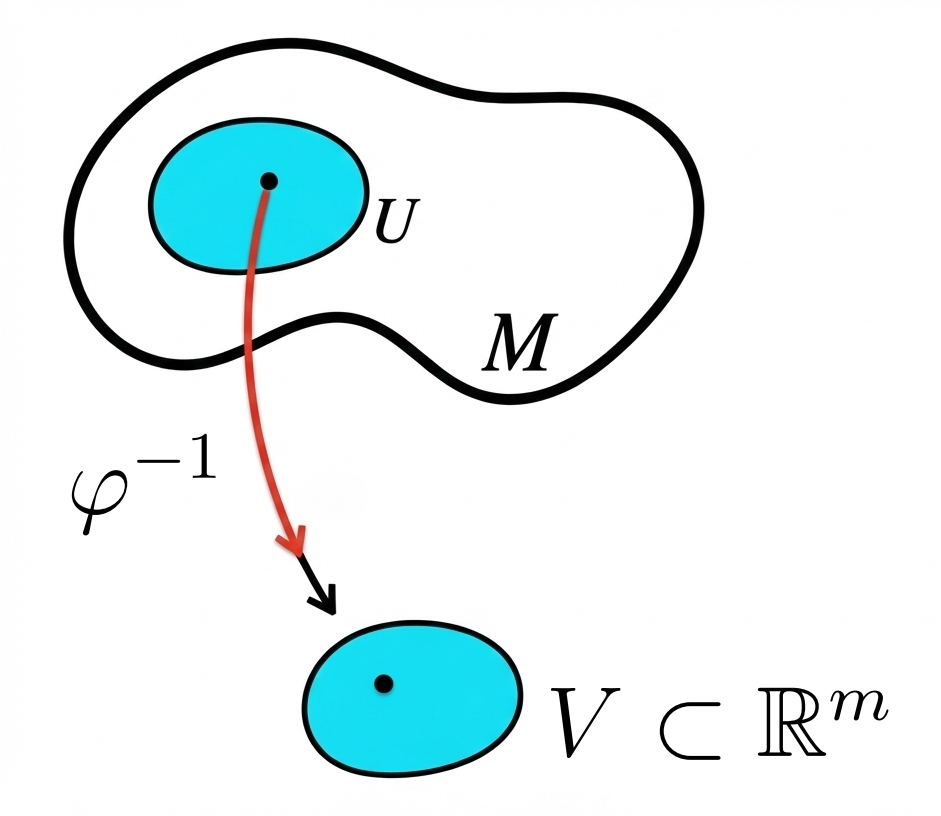
\includegraphics[width=0.3\textwidth, ]{Pictures/map.png}
		\caption{\raggedright Иллюстрация к определению многообразия.}
		\label{fig:map}
\end{framed}
\end{figure}
\end{definition}




\begin{note}
	По сути определение говорит, что $M$ является $m$-мерным многообразием, если в окрестности каждой своей точки напоминает открытое подмножество $\R^m$. Это отражено в определении $\phi$.
\end{note}

\begin{example}
	Рассмотрим плоскость $\Pi \subset \R^3$, $p = (x_0, y_0, z_0) \in \Pi$, параллельную линейно независимым векторам $a = (a_1, b_1, c_1)$, $b = (a_2, b_2, c_2)$. 
	Утверждается, что $\Pi$ является гладким двумерным многообразием. 
	Действительно, любая точка $q = (x, y, z) \in \Pi$ представляется в виде 
	\[ (x, y, z) = (x_0, y_0, z_0) + u \cdot (a_1, b_1, c_1) + v \cdot (a_2, b_2, c_2), \quad u, v \in \R. \] 
	Естественно возникает $\phi(u, v) = p + ua + vb$. Возьмем $V = \R^2$, $W = \R^3$, $M = \Pi$.
	Легко убедиться, что все условия локальной параметризации удовлетворяются.  
\end{example}

\begin{example}
	Рассмотрим $S^2 = \{(x, y, z) : x^2+y^2+z^2 = 1\}$. Утверждается, что $S^2$ является гладким двумерным многообразием.
	В качестве локальной параметризации возьмем 
	\[ \phi(\theta, \psi) = (\cos \theta \cos \psi, \sin \theta \cos \psi, \sin \psi), \quad V = (0, 2\pi) \times (-\pi/2, \pi/2). \]
	Это гомеоморфизм между $V$ и почти всей сферой $S^2$, за исключением главного меридиана (точек в плоскости $Oxz$, $x \ge 0$). 
	Для точек на вырезанном меридиане можно построить аналогичную параметризацию, повернув систему координат. 
\end{example}

\begin{problem}
	Покажите, что $M \subset \R^n$ является гладким $n$-мерным многообразием тогда и только тогда, когда $M$ открыто.
\end{problem}

\begin{example}
	Пусть $V$ открыто в $\R^m$ и $f : V \to \R^{n-m}$ гладкая. Тогда график $\Gamma_f = \{(x, f(x)) : x \in V\}$ является гладким $m$-мерным многообразием в $\R^n$. 
\end{example}

\begin{myproof}
	Рассмотрим $\phi : V \to \R^n$, $\phi(x) = (x, f(x))$. Тогда $\phi$ -- гладкая, $D \phi$ имеет ранг $m$ на $V$, а обратное отображение $\psi : \Gamma_f \to V$, $\psi(x, f(x)) = x$, непрерывно. 
	Следовательно, $\phi$ является параметризацией $\Gamma_f$ в окрестности каждой точки.
\end{myproof}

\vspace{5pt}
Следующая теорема дает иные способы описания гладких многообразий.

\begin{theorem}
	Пусть $M \subset \R^n$ и $0 < m < n$. Следующие утверждения эквивалентны: 
	\begin{enumerate}[itemsep = 0pt, topsep = 5pt]
		\item $M$ -- гладкое $m$-мерное многообразие в $\R^n$, 
		\item $\forall p \in M$ найдутся открытые в $\R^n$ множества $U \ni p$, $W$ и диффеоморфизм $\Phi : U \to W$, такие что $\Phi(M \cap U) = W \cap (\R^m \times \{0\})$ (\textbf{выпрямляющий} диффеоморфизм),
		\item $\forall p \in M$ найдутся открытое в $\R^n$ множество $U \ni p$ и такая гладкая функция $F : U \to \R^{n-m}$, что $M \cap U = F^{-1}(0)$ и $\operatorname{rk} DF(x) = n-m$ для всех $x \in M \cap U$
		(локальное задание многообразия уравнениями).
	\end{enumerate}
\end{theorem}

\begin{myproof}
	$(1 \Ra 2)$ Пусть $\phi : V \to \R^n$ -- локальная параметризация в окрестности $p = \phi(a) \in M$.
	По условию столбцы матрицы $D\phi(a)$ линейно независимы. %, дополним их до базиса $\R^n$. 
	Следовательно, найдется такая матрица $A$ размера $n \times (n-m)$, что $\det (D\phi(a) | A) \neq 0$.
	Определим $F : V \times \R^{n-m} \to \R^n$, $F(x, y) = \phi(x) + Ay$, тогда $F$ гладкая и $DF(a, 0) = (D\phi(a)|A)$ невырождена. 
	Поэтому по теореме об обратной функции найдутся окрестность $\widetilde{V} \subset V \times \R^{n-m}$ точки $(a, 0)$ и $\widetilde{U} \ni p$ открытое в $\R^n$, такие что $F : \widetilde{V} \to \widetilde{U}$ является диффеоморфизмом.

	\vspace{5pt}
	Пусть $V_0 = \{x \in \R^m : (x, 0) \in \widetilde{V}\}$. Тогда $V_0$ открыто в $\R^m$, а значит, $\phi(V_0) = F(V_0 \times \{0\})$ открыто в $M$ как образ открытого множества при гомеоморфизме $\phi$.
	Найдется такое открытое $U_0 \subset \R^n$, что $M \cap U_0 = \phi(V_0)$.
	Положим $U = U_0 \cap \widetilde{U}$, $W = F^{-1}(U)$, $\Phi = F^{-1}$.
	Отображение $\Phi : U \to W$ искомое. 
	Действительно, $\Phi$ диффеоморфизм как сужение $F^{-1}$ и 
	\[ \Phi(M \cap U) = \Phi(\phi(V_0)) = F^{-1}(F(V_0 \times \{0\})) = V_0 \times \{0\} = W \cap (\R^m \times \{0\}). \]
	Здесь $M \cap (U_0 \cap \widetilde{U}) \equiv M \cap U_0$, поскольку $M \cap U_0 = F(V_0 \times \{0\}) \subset \widetilde{U}$, 
	а последнее равенство можно показать двумя включениями: $V_0 \times \{0\} = \widetilde{V} \cap (\R^m \times \{0\}) = F^{-1}(\widetilde{U}) \cap (\R^m \times \{0\}) \supset W \cap (\R^m \times \{0\})$ и $V_0 \times \{0\} = \Phi(M \cap U) \cap (\R^m \times \{0\}) \subset \Phi(U) \cap (\R^m \times \{0\}) = W \cap (\R^m \times \{0\})$.

	\vspace{5pt}
	$(2 \Ra 3)$ Пусть $\Phi = (\Phi_1, \dotsc, \Phi_n) : U \to W$ -- диффеоморфизм из $(2)$. 
	Положим $F = (\Phi_{m+1}, \dotsc, \Phi_n)$, тогда $x \in M \cap U \iff F(x) = 0$ и $\operatorname{rk} DF = n-m$ на $M \cap U$.

	\vspace{5pt}
	$(3 \Ra 1)$ Зафиксируем $p \in M$. Будем предполагать, что в матрице $DF(p)$ независимы последние $n-m$ столбцов, иначе заменим $F$ на композицию с перестановкой. 
	Запишем $\R^n = \R^m_x \times \R^{n-m}_y$, $p = (a, b)$. 
	Тогда $\frac{\partial F}{\partial y}(p)$ невырождена и $(x, y) \in M \cap U \iff F(x, y) = 0$. 
	По теореме о неявной функции найдутся окрестности $V' \ni a$ и $V'' \ni b$ (настолько малые, что $V_0 = V' \times V'' \subset U$) 
	и такая гладкая $f: V' \to \R^{n-m}$, что 
	\[ M \cap V_0 = \{(x, y) \in V_0 : F(x, y) = 0\} = \{(x, f(x)) : x \in V'\} = \Gamma_f. \]
	Осталось воспользоваться предыдущим примером.
\end{myproof}

\begin{example}
	$S^{n-1} = \{x \in \R^n : |x| = 1\}$ -- гладкое $(n-1)$-мерное многообразие в $\R^n$.
\end{example}

\begin{myproof}
	Действительно, функция $F : \R^n \setminus \{0\} \to \R$, $F(x) = |x|^2 - 1$ гладкая, градиент $\nabla F(x) = 2x \neq 0$ и $S^{n-1} = F^{-1}(0)$. 
	Осталось применить третий пункт теоремы.
\end{myproof}

\begin{problem}
	Пусть $A$ -- ненулевая симметрическая матрица порядка $n$ и $c \neq 0$.
	Докажите, что $M = \{x \in \R^n : x^T A x = c\}$ -- гладкое $(n-1)$-мерное многообразие. 
	Приведите пример, что при $c = 0$ множество $M$ может не быть гладким многообразием.
\end{problem}

\subsection{Гладкие отображения по Милнору}

Обобщим, следуя Милнору, понятие гладкости отображения на отображения произвольных (необязательно открытых) множеств.

\begin{definition}
	Пусть $X \subset \R^n$, $Y \subset \R^l$ и $f : X \to Y$. 
	Отображение $f$ называется \textit{гладким} (\textit{по Милнору}), если $\forall x \in X : \exists U \ni x$ открытое в $\R^n$ и 
	гладкая функция $F : U \to \R^l$, такая что $F|_{X \cap U} = f|_{X \cap U}$. 
	$F$ называется \textit{гладким продолжением} $f$ в окрестности $x$.
\end{definition}

\begin{note}
	Отметим, что если $f : X \to Y$, $g : Y \to Z$ гладкие, то $g \circ f : X \to Z$ гладкое.
\end{note}

\begin{lemma}
	Пусть $M$ -- гладкое $m$-мерное многообразие в $\R^n$. Если $\phi: V \to \R^n$ -- локальная параметризация в окрестности $p$, 
	$\phi(V) = U_0$, то карта $\phi^{-1} : U_0 \to V$ гладкая.
\end{lemma}

\begin{myproof}
	Из доказательства пункта $(2)$ теоремы 3.1 следует, что диффеоморфизм $\Phi : U \to W$ можно выбрать так, что $M \cap U \subset U_0$. 
	Тогда $\Phi(q) = (\phi^{-1}(q), 0)$ для всех $q \in M \cap U$ (равенство очевидно, если подействовать $F$ на обе его части). 
	Сужая $W$, если необходимо, можно считать, что $W = W' \times W''$, где $W'$ открыто в $\R^m$, $W''$ открыто в $\R^{n-m}$. 
	Пусть $\pi : W \to W'$, $\pi(x, y) = x$ -- проектирование на $W'$. 
	Положим $F = \pi \circ \Phi$. Тогда $F$ гладкая и $F|_{M \cap U} = \phi^{-1}|_{M \cap U}$.
	Поскольку такие рассуждения можно провести в окрестности каждой точки из $U_0$, это доказывает, что $\phi^{-1}$ гладкая по Милнору. 
\end{myproof}

\begin{corollary}
	Карта $\phi^{-1}$ локально липшицева, то есть 
	$\forall p \in U_0 \ \exists C > 0$ и открытое в $M$ множество $W_0 \subset U_0$ ($p \in W_0$), что $\forall x, y \in W_0 : |\phi^{-1}(x) - \phi^{-1}(y)| \leq C |x-y|$. 
\end{corollary}

\begin{myproof}
	Рассмотрим гладкое продолжение $F = (F_1, \dotsc, F_n)$ функции $\phi^{-1}$ в окрестности $p$. 
	Тогда частные производные $\frac{\partial F_i}{\partial x_j}$ ограничены в некотором шаре $B$ с центром в $p$. 
	По лемме 2.1 найдется $C > 0$, что $\forall x, y \in B : |F(x) - F(y)| \leq C |x-y|$. 
	Следовательно, $\forall x, y \in B \cap U_0 =: W_0 : |\phi^{-1}(x) - \phi^{-1}(y)| \leq C |x-y|$.
\end{myproof}

\begin{definition}
	Пусть $M \subset \R^n$, $N \subset \R^m$ -- гладкие многообразия. 
	Отображение $f: M \to N$ называется \textit{диффеоморфизмом}, если $f$ -- биекция, $f$ и $f^{-1}$ гладкие по Милнору.
\end{definition}

\begin{corollary}
	Пусть $\phi : V \to \R^n$ локальная параметризация $M$ в окрестности $p$, $\phi(V) = U_0$.
	Тогда $\phi : V \to U_0$ является диффеоморфизмом по доказанной лемме. 
\end{corollary}

\begin{note}
	Таким образом, параметризация вводит криволинейные координаты в $U_0$. 
	Точке $q \in U_0$ сопоставляются координаты $(u_1, \dotsc, u_m)$ точки $\phi^{-1}(q)$ в $\R^m$.
\end{note}

\begin{corollary}[\textbf{о функциях перехода}]
	Пусть $\phi: V \to \R^n$, $\psi : W \to \R^n$ -- локальные параметризации $M$, $O = \phi(V) \cap \psi(W) \neq \emptyset$. 
	Тогда $g : \psi^{-1}(O) \to \phi^{-1}(O)$, $g = \phi^{-1} \circ \psi$ является диффеоморфизмом.
\end{corollary}

\begin{myproof}
	Так как $\phi$ и $\psi$ биекции, то $g$ также является биекцией. Функции $g = \phi^{-1} \circ \psi$ и $g^{-1} = \psi^{-1} \circ \phi$ являются гладкими по доказанной лемме.
\end{myproof}